% Options for packages loaded elsewhere
\PassOptionsToPackage{unicode}{hyperref}
\PassOptionsToPackage{hyphens}{url}
%
\documentclass[
]{article}
\usepackage{amsmath,amssymb}
\usepackage{iftex}
\ifPDFTeX
  \usepackage[T1]{fontenc}
  \usepackage[utf8]{inputenc}
  \usepackage{textcomp} % provide euro and other symbols
\else % if luatex or xetex
  \usepackage{unicode-math} % this also loads fontspec
  \defaultfontfeatures{Scale=MatchLowercase}
  \defaultfontfeatures[\rmfamily]{Ligatures=TeX,Scale=1}
\fi
\usepackage{lmodern}
\ifPDFTeX\else
  % xetex/luatex font selection
\fi
% Use upquote if available, for straight quotes in verbatim environments
\IfFileExists{upquote.sty}{\usepackage{upquote}}{}
\IfFileExists{microtype.sty}{% use microtype if available
  \usepackage[]{microtype}
  \UseMicrotypeSet[protrusion]{basicmath} % disable protrusion for tt fonts
}{}
\makeatletter
\@ifundefined{KOMAClassName}{% if non-KOMA class
  \IfFileExists{parskip.sty}{%
    \usepackage{parskip}
  }{% else
    \setlength{\parindent}{0pt}
    \setlength{\parskip}{6pt plus 2pt minus 1pt}}
}{% if KOMA class
  \KOMAoptions{parskip=half}}
\makeatother
\usepackage{xcolor}
\usepackage[margin=1in]{geometry}
\usepackage{longtable,booktabs,array}
\usepackage{calc} % for calculating minipage widths
% Correct order of tables after \paragraph or \subparagraph
\usepackage{etoolbox}
\makeatletter
\patchcmd\longtable{\par}{\if@noskipsec\mbox{}\fi\par}{}{}
\makeatother
% Allow footnotes in longtable head/foot
\IfFileExists{footnotehyper.sty}{\usepackage{footnotehyper}}{\usepackage{footnote}}
\makesavenoteenv{longtable}
\usepackage{graphicx}
\makeatletter
\def\maxwidth{\ifdim\Gin@nat@width>\linewidth\linewidth\else\Gin@nat@width\fi}
\def\maxheight{\ifdim\Gin@nat@height>\textheight\textheight\else\Gin@nat@height\fi}
\makeatother
% Scale images if necessary, so that they will not overflow the page
% margins by default, and it is still possible to overwrite the defaults
% using explicit options in \includegraphics[width, height, ...]{}
\setkeys{Gin}{width=\maxwidth,height=\maxheight,keepaspectratio}
% Set default figure placement to htbp
\makeatletter
\def\fps@figure{htbp}
\makeatother
\setlength{\emergencystretch}{3em} % prevent overfull lines
\providecommand{\tightlist}{%
  \setlength{\itemsep}{0pt}\setlength{\parskip}{0pt}}
\setcounter{secnumdepth}{-\maxdimen} % remove section numbering
\newlength{\cslhangindent}
\setlength{\cslhangindent}{1.5em}
\newlength{\csllabelwidth}
\setlength{\csllabelwidth}{3em}
\newlength{\cslentryspacingunit} % times entry-spacing
\setlength{\cslentryspacingunit}{\parskip}
\newenvironment{CSLReferences}[2] % #1 hanging-ident, #2 entry spacing
 {% don't indent paragraphs
  \setlength{\parindent}{0pt}
  % turn on hanging indent if param 1 is 1
  \ifodd #1
  \let\oldpar\par
  \def\par{\hangindent=\cslhangindent\oldpar}
  \fi
  % set entry spacing
  \setlength{\parskip}{#2\cslentryspacingunit}
 }%
 {}
\usepackage{calc}
\newcommand{\CSLBlock}[1]{#1\hfill\break}
\newcommand{\CSLLeftMargin}[1]{\parbox[t]{\csllabelwidth}{#1}}
\newcommand{\CSLRightInline}[1]{\parbox[t]{\linewidth - \csllabelwidth}{#1}\break}
\newcommand{\CSLIndent}[1]{\hspace{\cslhangindent}#1}

\usepackage{amsmath}
\usepackage{nomencl}
\makenomenclature 


%\usepackage{booktabs}
%\usepackage{longtable}
%\usepackage{morefloats}
%\extrafloats{100}
%\date{August 25, 2021}
%\renewcommand{\today}{September 5, 2021}

% Set the copyright footer
%\lfoot{\copyright 2021 P.J. Palmer  P.M. Leonard}

% Some figure placement options.
%\usepackage[figuresonly,nomarkers,fighead, figlist]{endfloat}
%\usepackage[figuresonly,nomarkers,nolists]{endfloat}
% Put multiple figures per page
%\renewcommand{\efloatseparator}{\mbox{}}
\usepackage{flafter}
\ifLuaTeX
  \usepackage{selnolig}  % disable illegal ligatures
\fi
\IfFileExists{bookmark.sty}{\usepackage{bookmark}}{\usepackage{hyperref}}
\IfFileExists{xurl.sty}{\usepackage{xurl}}{} % add URL line breaks if available
\urlstyle{same}
\hypersetup{
  pdftitle={Experiments with a Berlese Funnel},
  pdfauthor={Paul J. Palmer},
  hidelinks,
  pdfcreator={LaTeX via pandoc}}

\title{Experiments with a Berlese Funnel}
\author{Paul J. Palmer}
\date{}

\begin{document}
\maketitle

Trying to figure out what to call a Berlese (or Tullgren) Funnel takes more time than describing what it does. It is an apparatus for collecting microfauna from soil or leaf litter samples. The history is hard to pin down, but the earliest mention seems to be from Berlese (1905) and Tullgren (1917) so it appears that Berlese was the first to describe the apparatus, using a water bath as a heater, and then Tullgren simplified the overall arrangement by using an electric lamp as a source of heat. I'm going to stick with ``Berlese Funnel'' for now.

The general principle involves providing a funnel with a fine-mesh lid, an inner coarse mesh upon which the sample material is laid, and a slippery funnel leading to a receptacle with a liquid preserving agent. The use of a lamp to warm and dry the sample is an optional extra in these days of high energy costs, especially if you keep the apparatus in a warm, dry place. Mine was set up in the greenhouse with a small lamp to dry the material (See Figure \ref{fig:BerleseFunnel}) and a tube filled with 100\% Mono Propylene Glycol (MPG) to catch the microfauna. I'm a fan of MPG as it is a good preservative, slow to evaporate, non toxic, preserves colours, and keeps specimens fairly supple. I found that most of the catch appeared after three days and little ever appeared after a week.

\begin{figure}

{\centering 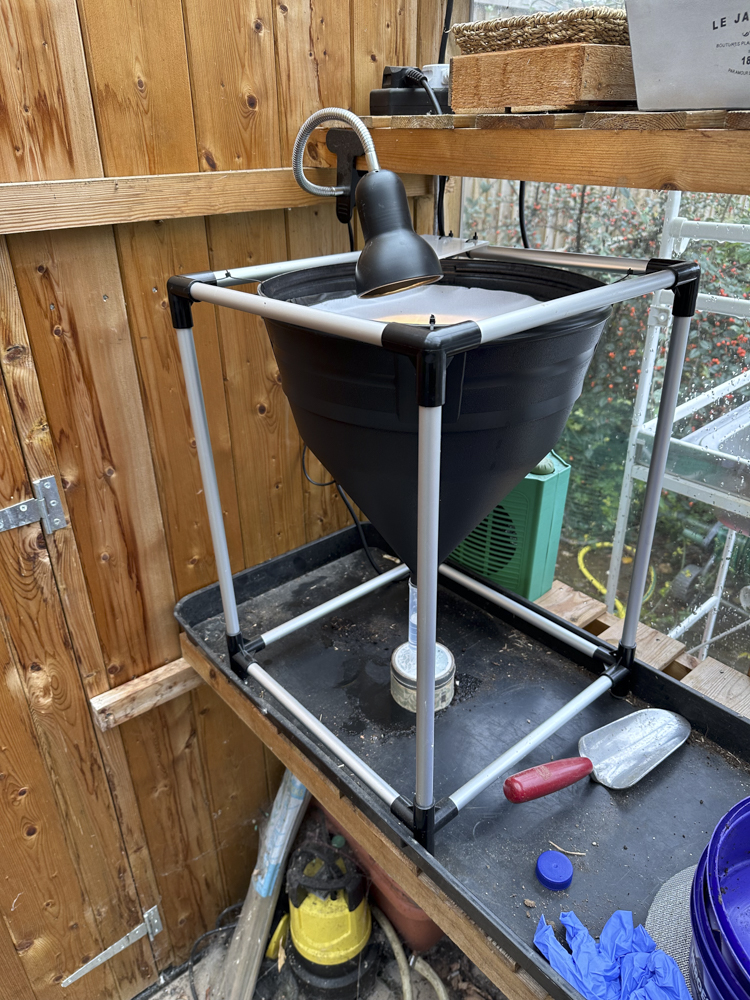
\includegraphics[width=0.8\linewidth]{images/BerleseFunnel} 

}

\caption{Berlese Funnel set up in the greenhouse.}\label{fig:BerleseFunnel}
\end{figure}

For my experimental trial, all the material came from locations on the nature reserve at Rutland Water: So what did I find?

My favourite and a personal first was the Pseudoscorpion \emph{Chthonius ischnocheles} (Common Chthonid) Figure \ref{fig:ChthoniusIschnocheles}. It turned out that the keys to woodlice are quite easy to use so Figures \ref{fig:TrichoniscusPusillus} and \ref{fig:PhilosciaMuscorum} show the common woodlice \textit{Trichoniscus pusillus} Ag. and \textit{Philoscia muscorum}. All the by-catch was separated and logged.

Oxypselaphus obscurus X2
Agonum fuliginosum X3
Anotylus rugosus X2
Stenolophus mixtus X1
Acupalpus dubius X1
Octhebius pusillus X1 - just 1 previous record 1936 (STET Ochthebius pusillus)
Dacrila fallax X1 - 3 previous records, last Rutland Water 2021
Habrocerus capillaricornis X1
Lathrobium brunnipes X1

After this encouraging start I shall be expanding

\begin{figure}

{\centering 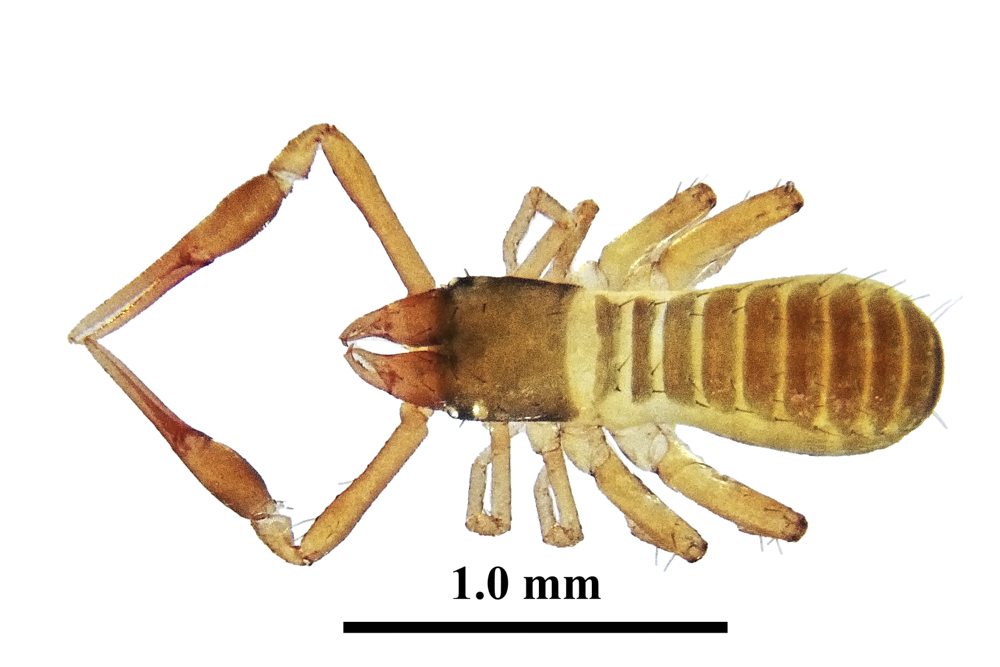
\includegraphics[width=0.8\linewidth]{images/ChthoniusIschnocheles} 

}

\caption{ \textit{Chthonius ischnocheles} Common Chthonid  }\label{fig:ChthoniusIschnocheles}
\end{figure}

\begin{figure}

{\centering 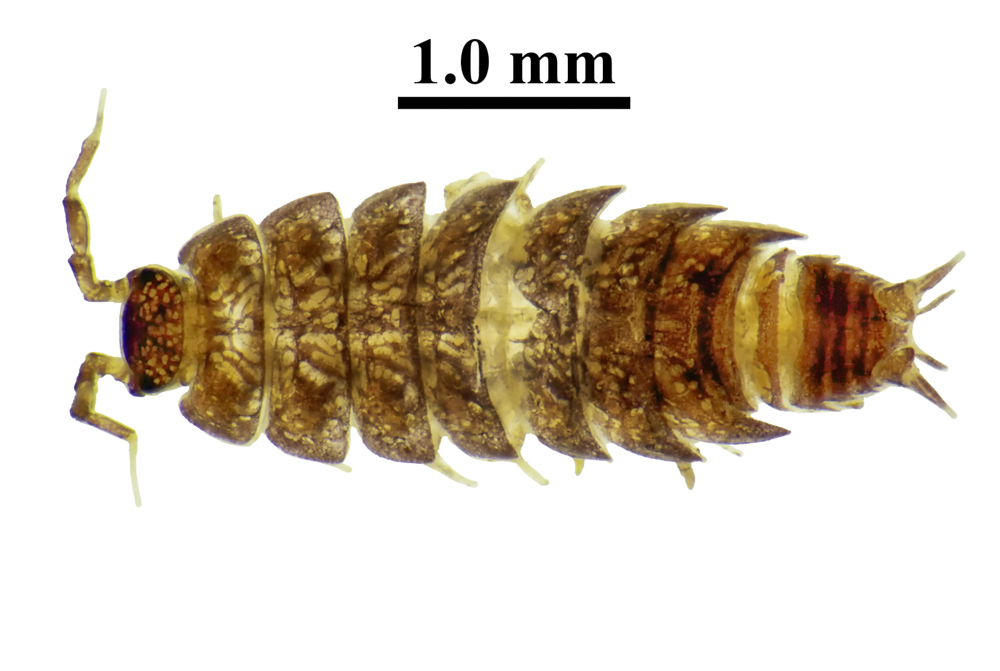
\includegraphics[width=0.8\linewidth]{images/TrichoniscusPusillus} 

}

\caption{  \textit{Trichoniscus pusillus} Ag. Common Pygmy Woodlouse}\label{fig:TrichoniscusPusillus}
\end{figure}

\begin{figure}

{\centering 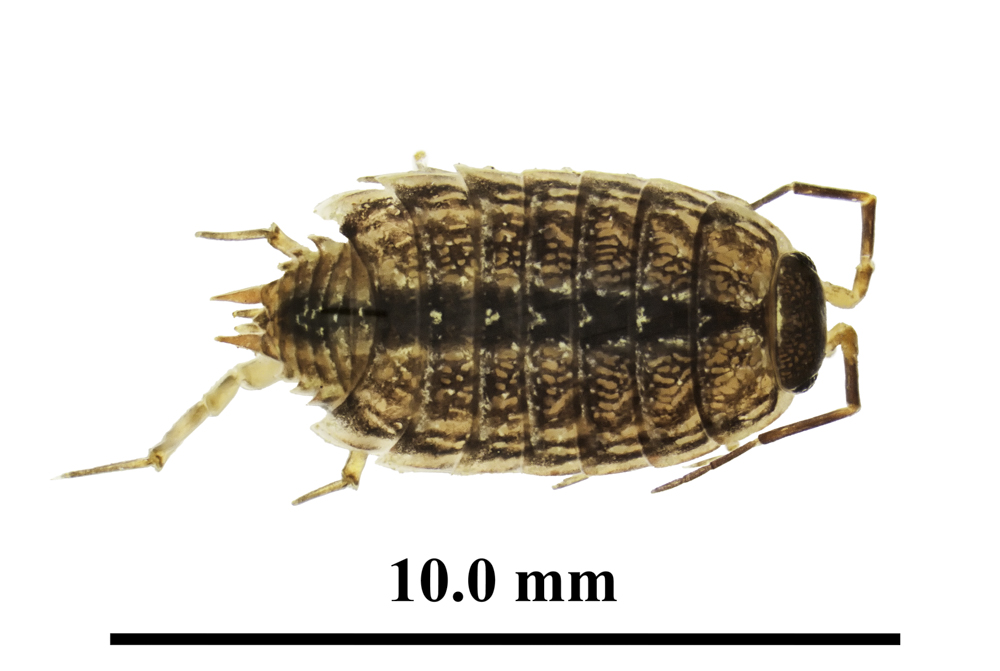
\includegraphics[width=0.8\linewidth]{images/PhilosciaMuscorum} 

}

\caption{\textit{Philoscia muscorum} Common Striped Woodlouse}\label{fig:PhilosciaMuscorum}
\end{figure}

\begin{figure}

{\centering 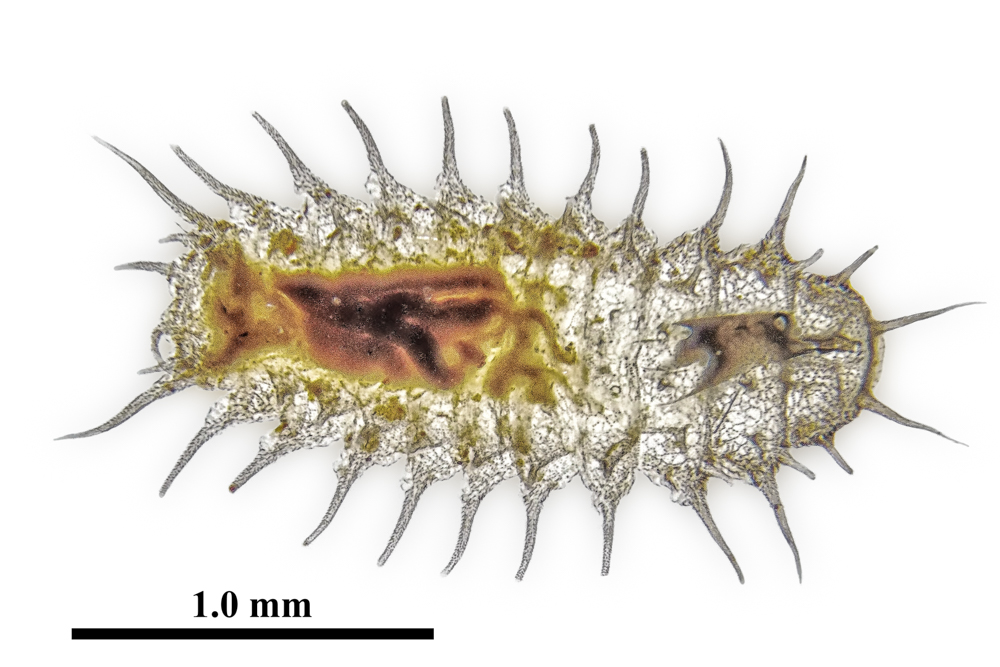
\includegraphics[width=0.8\linewidth]{images/Coccinid} 

}

\caption{Unknown \textit{Coccinid} Scale Insect, mobile stage.}\label{fig:Coccinid}
\end{figure}

\newpage

\hypertarget{bibliography}{%
\section*{Bibliography}\label{bibliography}}
\addcontentsline{toc}{section}{Bibliography}

This short bibliography covers sources that helped to inspire this article.

\hypertarget{refs}{}
\begin{CSLReferences}{1}{0}
\leavevmode\vadjust pre{\hypertarget{ref-Berlese1905}{}}%
Berlese, Antonio. 1905. {``Apparecchio Per Raccogliere Presto e in Gran Numero Piccoli Arthropodi.''} \emph{REDIA -- Journal of Zoology}, 85--89.

\leavevmode\vadjust pre{\hypertarget{ref-Tullgren1917}{}}%
Tullgren, A. 1917. {``En Enkel Apprat För Automatiskt Vittjande Av Sällgods.''} \emph{Entomologisk Tidskrift} 38: 97--100. \url{https://www.biodiversitylibrary.org/item/42375\#page/124/mode/1up}.

\end{CSLReferences}

\let\cleardoublepage\clearpage

\end{document}
